\documentclass[10pt]{article}
\usepackage[utf8]{inputenc}
\usepackage[T1]{fontenc}
\usepackage{amsmath}
\usepackage{amsfonts}
\usepackage{amssymb}
\usepackage[version=4]{mhchem}
\usepackage{stmaryrd}
\usepackage{graphicx}
\usepackage[export]{adjustbox}
\graphicspath{ {./images/} }

\title{Università di Catania 
 Corso di Laurea in Fisica 
 Compito scritto di Fisica Generale I 
 M.G. Grimaldi - A. Insolia }

\author{}
\date{}


\begin{document}
\maketitle
Catania, 13 Luglio 2022

Per la prova in itinere ( 2 ore) svolgere i problemi: \(3,4,5\)

Per la prova completa (3 ore) svolgere i problemi: \(1,2,3,4\)

\section{Problema n.1}
Come mostrato in figura, una guida è costituita da un tratto verticale rettilineo e da un arco di circonferenza di raggio \(\mathrm{R}=50.0 \mathrm{~cm}\); la parte destra dell'arco di circonferenza ha un apertura (rispetto alla verticale) di \(\pi / 3\). Affiancata alla guida vi è un tratto rettilineo orizzontale di lunghezza \(\mathrm{L}=3 \mathrm{R}\) (dal punto \(\mathrm{P}\) al punto \(\mathrm{Q}\) ) alla quota del punto più basso della guida. Un punto materiale di massa m viene lasciato libero (in quiete) da un punto della guida ad una quota iniziale \(\mathrm{h}\) (misurata dal punto più basso della guida); il corpo, dopo aver scivolato lungo la guida stessa, cadrà (dopo un breve volo) sul tratto orizzontale. Trascurando ogni tipo di attrito (sia con la guida che con l'aria), determinare:

a) il valore di \(h, h_{P}\), affinchè il punto materiale cada nel punto \(P\);

b) il valore di \(h, h_{Q}\), affinchè il punto materiale cada nel punto \(Q\);

c) la massima quota raggiunta dal punto materiale durante il suo volo nel caso di \(h=R\).

\begin{center}
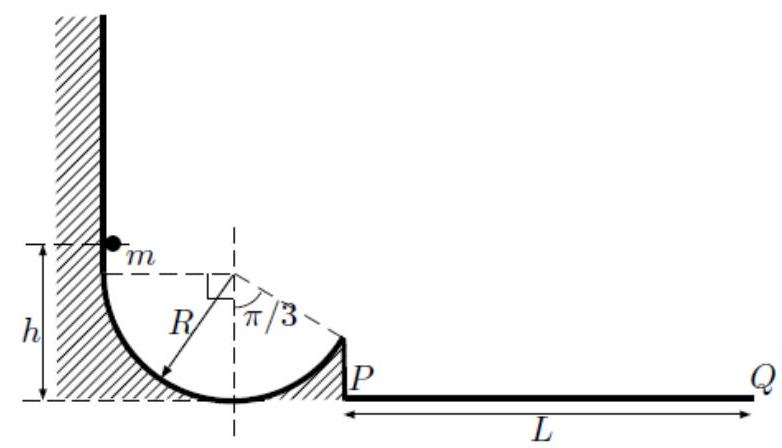
\includegraphics[max width=\textwidth]{2023_05_14_f410bf68b032e0bd342dg-1}
\end{center}

\section{Problema n.2}
Si abbia (come schematizzato in figura) un corpo rigido a forma di T rovesciata di massa \(\mathrm{M}=4 \mathrm{~m}\). La T rovesciata è costituita da due barre sottili identiche di lunghezza I=100 cm e massa \(2 \mathrm{~m}\), con il centro della seconda saldata ad uno degli estremi della prima. Come mostra la figura, l'altro estremo della prima barra è imperniato ad una asse orizzontale intorno a cui la T può ruotare liberamente; inoltre, dalla figura si vede che ad uno degli estremi della seconda barra è appeso, tramite un filo di massa trascurabile, un corpo di massa \(m\).

a) Pensando il sistema in equilibrio statico determinare l'angolo \(\theta_{0}\) (vedi figura) che la prima barra della T rovesciata forma con la verticale.

b) Supponendo poi che il filo che sostiene il corpo di massa \(m\) venga tagliato, si determini il periodo delle oscillazioni che la T rovesciata inizierebbe a fare (data la piccola ampiezza di queste, si considerino le oscillazioni come piccole).

\begin{center}
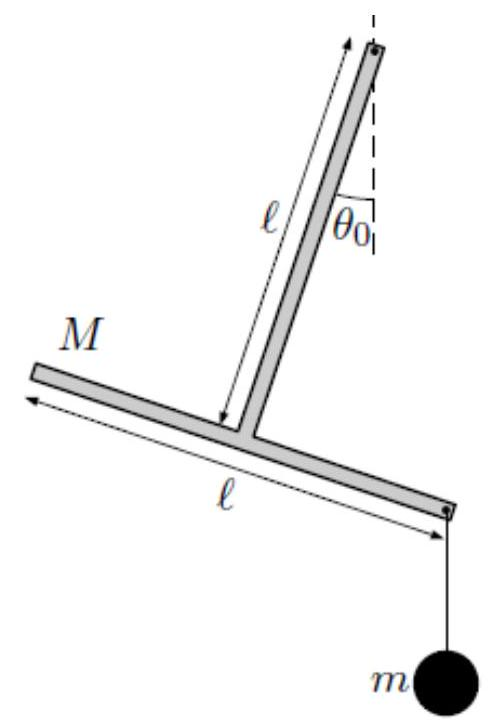
\includegraphics[max width=\textwidth]{2023_05_14_f410bf68b032e0bd342dg-2}
\end{center}

\section{Problema n.3}
Un cubo omogeneo di lato \(10 \mathrm{~cm}\) e densità \(0.7 \mathrm{~g} / \mathrm{cm}^{3}\) viene posto (con velocità nulla) sul fondo di un contenitore pieno d' acqua. L' altezza del liquido è un metro.

a) Calcolare la velocità con cui la faccia superiore del cubo raggiunge il pelo libero superiore dell'acqua.

b) Se il cubo fosse attaccato al fondo tramite una molla di lunghezza a riposo nulla e \(k=10 \mathrm{~N} / \mathrm{m}\), quale sarebbe l'elongazione massima della molla?

\section{Problema n.4}
Una mole di un gas perfetto monoatomico compie un ciclo termodinamico reversibile. A partire dallo stato di equilibrio 1 con \(p_{1}=1\) bar, \(T_{1}=300 \mathrm{~K}\), vengono eseguite le seguenti trasformazioni in sequenza: espansione isobara fino allo stato 2 ed espansione adiabatica fino allo stato 3, quindi compressione isoterma per riportare il gas allo stato iniziale.

a) Determinare il volume occupato dal gas negli stati 2 e 3 , se il calore assorbito totale è pari a \(\mathrm{Q}_{\mathrm{a}}=2000 \mathrm{~J}\).

b) Determinare il rendimento del ciclo.

\section{Problema n.5}
Un calorimetro è composto da un recipiente contenente acqua, isolato termicamente dall'ambiente esterno e riscaldato con un dispositivo che fornisce un potenza \(\mathrm{P}=45 \mathrm{~W}\). Il tempo necessario a portare il sistema dalla temperatura ambiente \(T_{A}=20^{\circ} \mathrm{C}\) alla temperatura \(T_{B}=50{ }^{\circ} \mathrm{C}\) è pari a 20 minuti. Successivamente viene posto nel recipiente un corpo di massa \(m=100 \mathrm{~g}\) di un materiale di calore specifico incognito, misurando il tempo di riscaldamento da \(T_{A}\) a \(T_{B}\) si trova che ora esso é pari a \(1280 \mathrm{~s}\). Calcolare:

a) il calore specifico incognito della sostanza che costituisce il corpo;

b) la variazione di energia interna del sistema (calorimetro+materiale) e del materiale nel processo di riscaldamento;

c) la variazione di entropia del materiale quando viene raffreddato da \(50{ }^{\circ} \mathrm{C}\) a \(20^{\circ} \mathrm{C}\).


\end{document}